% Use only LaTeX2e, calling the article.cls class and 12-point type.

\documentclass[12pt]{article}

% Users of the {thebibliography} environment or BibTeX should use the
% scicite.sty package, downloadable from *Science* at
% www.sciencemag.org/about/authors/prep/TeX_help/ .
% This package should properly format in-text
% reference calls and reference-list numbers.

\usepackage{scicite}

% Use times if you have the font installed; otherwise, comment out the
% following line.

\usepackage{times}

% The preamble here sets up a lot of new/revised commands and
% environments.  It's annoying, but please do *not* try to strip these
% out into a separate .sty file (which could lead to the loss of some
% information when we convert the file to other formats).  Instead, keep
% them in the preamble of your main LaTeX source file.
\usepackage{graphicx}
\usepackage{subcaption}

% The following parameters seem to provide a reasonable page setup.

\topmargin 0.0cm
\oddsidemargin 0.2cm
\textwidth 16cm 
\textheight 21cm
\footskip 1.0cm


%The next command sets up an environment for the abstract to your paper.

\newenvironment{sciabstract}{%
\begin{quote} \bf}
{\end{quote}}


% If your reference list includes text notes as well as references,
% include the following line; otherwise, comment it out.

\renewcommand\refname{References and Notes}

% The following lines set up an environment for the last note in the
% reference list, which commonly includes acknowledgments of funding,
% help, etc.  It's intended for users of BibTeX or the {thebibliography}
% environment.  Users who are hand-coding their references at the end
% using a list environment such as {enumerate} can simply add another
% item at the end, and it will be numbered automatically.

\newcounter{lastnote}
\newenvironment{scilastnote}{%
\setcounter{lastnote}{\value{enumiv}}%
\addtocounter{lastnote}{+1}%
\begin{list}%
{\arabic{lastnote}.}
{\setlength{\leftmargin}{.22in}}
{\setlength{\labelsep}{.5em}}}
{\end{list}}


% Include your paper's title here

\title{Quality-of-Service (QoS) Esitmation in Software-Defined Networks\\
	\large Computer Networks II: Project Final Report} 


% Place the author information here.  Please hand-code the contact
% information and notecalls; do *not* use \footnote commands.  Let the
% author contact information appear immediately below the author names
% as shown.  We would also prefer that you don't change the type-size
% settings shown here.

\author
{Xin Liu\\
\\
\normalsize{Department of Computer Science, }\\
\normalsize{Illinois Institute of Technology, }\\
\normalsize{xliu125@hawk.iit.edu}\\
}
% Include the date command, but leave its argument blank.

\date{}



%%%%%%%%%%%%%%%%% END OF PREAMBLE %%%%%%%%%%%%%%%%



\begin{document} 

% Double-space the manuscript.

\baselineskip24pt

% Make the title.

\maketitle 




% In setting up this template for *Science* papers, we've used both
% the \section* command and the \paragraph* command for topical
% divisions.  Which you use will of course depend on the type of paper
% you're writing.  Review Articles tend to have displayed headings, for
% which \section* is more appropriate; Research Articles, when they have
% formal topical divisions at all, tend to signal them with bold text
% that runs into the paragraph, for which \paragraph* is the right
% choice.  Either way, use the asterisk (*) modifier, as shown, to
% suppress numbering.

\section{Introduction}

Multimedia applications have strict requirements of Quality-
of-Service (QoS) in order to guarantee user experience. Thus,
accurately measure the QoS metrics, such as throughput
and latency, is a critical task. However, packet-switching
network has the nature of multiplexed flows and best-effort
forwarding, which makes the task difficult to accomplish.
Software-Defined Networking (SDN) \cite{SDN} is a newly proposed
network architecture that separates the packet forwarding
(data plane) and control logic (control plane). The forward-
ing devices (i.e., switches) in SDN network keep simple data
structures and process schemes locally, while the centralized
entity (i.e., controller), which connects to all the forwarding
devices, maintains network states and execute complicated
control algorithm to operate the network. In addition to modifying the table entries on the switches, controller has the ability to pull the statistical information maintained by all the switches, which enables us to utilize these information to estimate the throughput of a flow. In this work, we use a simple formula to calculate the throughput, and conduct experiments to evaluate whether this calculation is close to the actual end-to-end throughput. By using network emulation and Linux iperf test, we verified that the estimated result is relatively accurate in a simple linear topology, and the accuracy is related to which switch is chosen to monitor. From the result, we find there is a potential research direction on how to choose the target switches in a large-scale complicated network.

The rest of this report is organized as follows: section 2 gives a brief background on SDN and related work; section 3 shows the simple formula we use to esitmate the flow throughput; the emulation tool and throughput measurement tool is introduced at section 4, followed by the desciption of experiment setup, then the result analysis; finally section 5 gives the conclusion of this study and propose a future work.

\section{Background and Related Work}
Software-Defined Network (SDN) is a network architecture composed of three layers: Infraustructure layer, Control layer, and Application layer. As shown in Figure \ref{fig:arch}, the lowest layer is infrastructure layer which is composed of hardware devices with simple forwarding tables and match-action packet processing mechanism. The middle layer, controller layer, contains a (logically) central entity (i.e., controller) that communicate with the low-level hardware and provide services to the upper applications. The "services" include topology information, flow statistics, shortest paths, etc. Network operators utilize these services to implement their network policies, and run as network applications at the top layer. While the communication protocol between Control layer and Application layer ("northbound API") has not been standardized yet, there is a widely adopted protocol between Control layer and Infrastructure layer ("southbound API"), named OpenFlow \cite{openflow}. OpenFlow-enabled devices contain a pipeline of forwarding tables, each of which contains a number of table entries shown in Figure \ref{fig:openflow}. The match field contains a set of values to identify the incoming packets to process, which means to apply the action specified by the action field. Meanwhile, for every packet that is matched by this entry, the corresponding stats field is going to be updated. The controller is able to install/remove/update the entries on all the switches using the OpenFlow protocol, while the switches can notify the controller about certain events, such as the arrival of new (unmatched) packet, link failure, etc. 

\begin{figure}
  \centering
  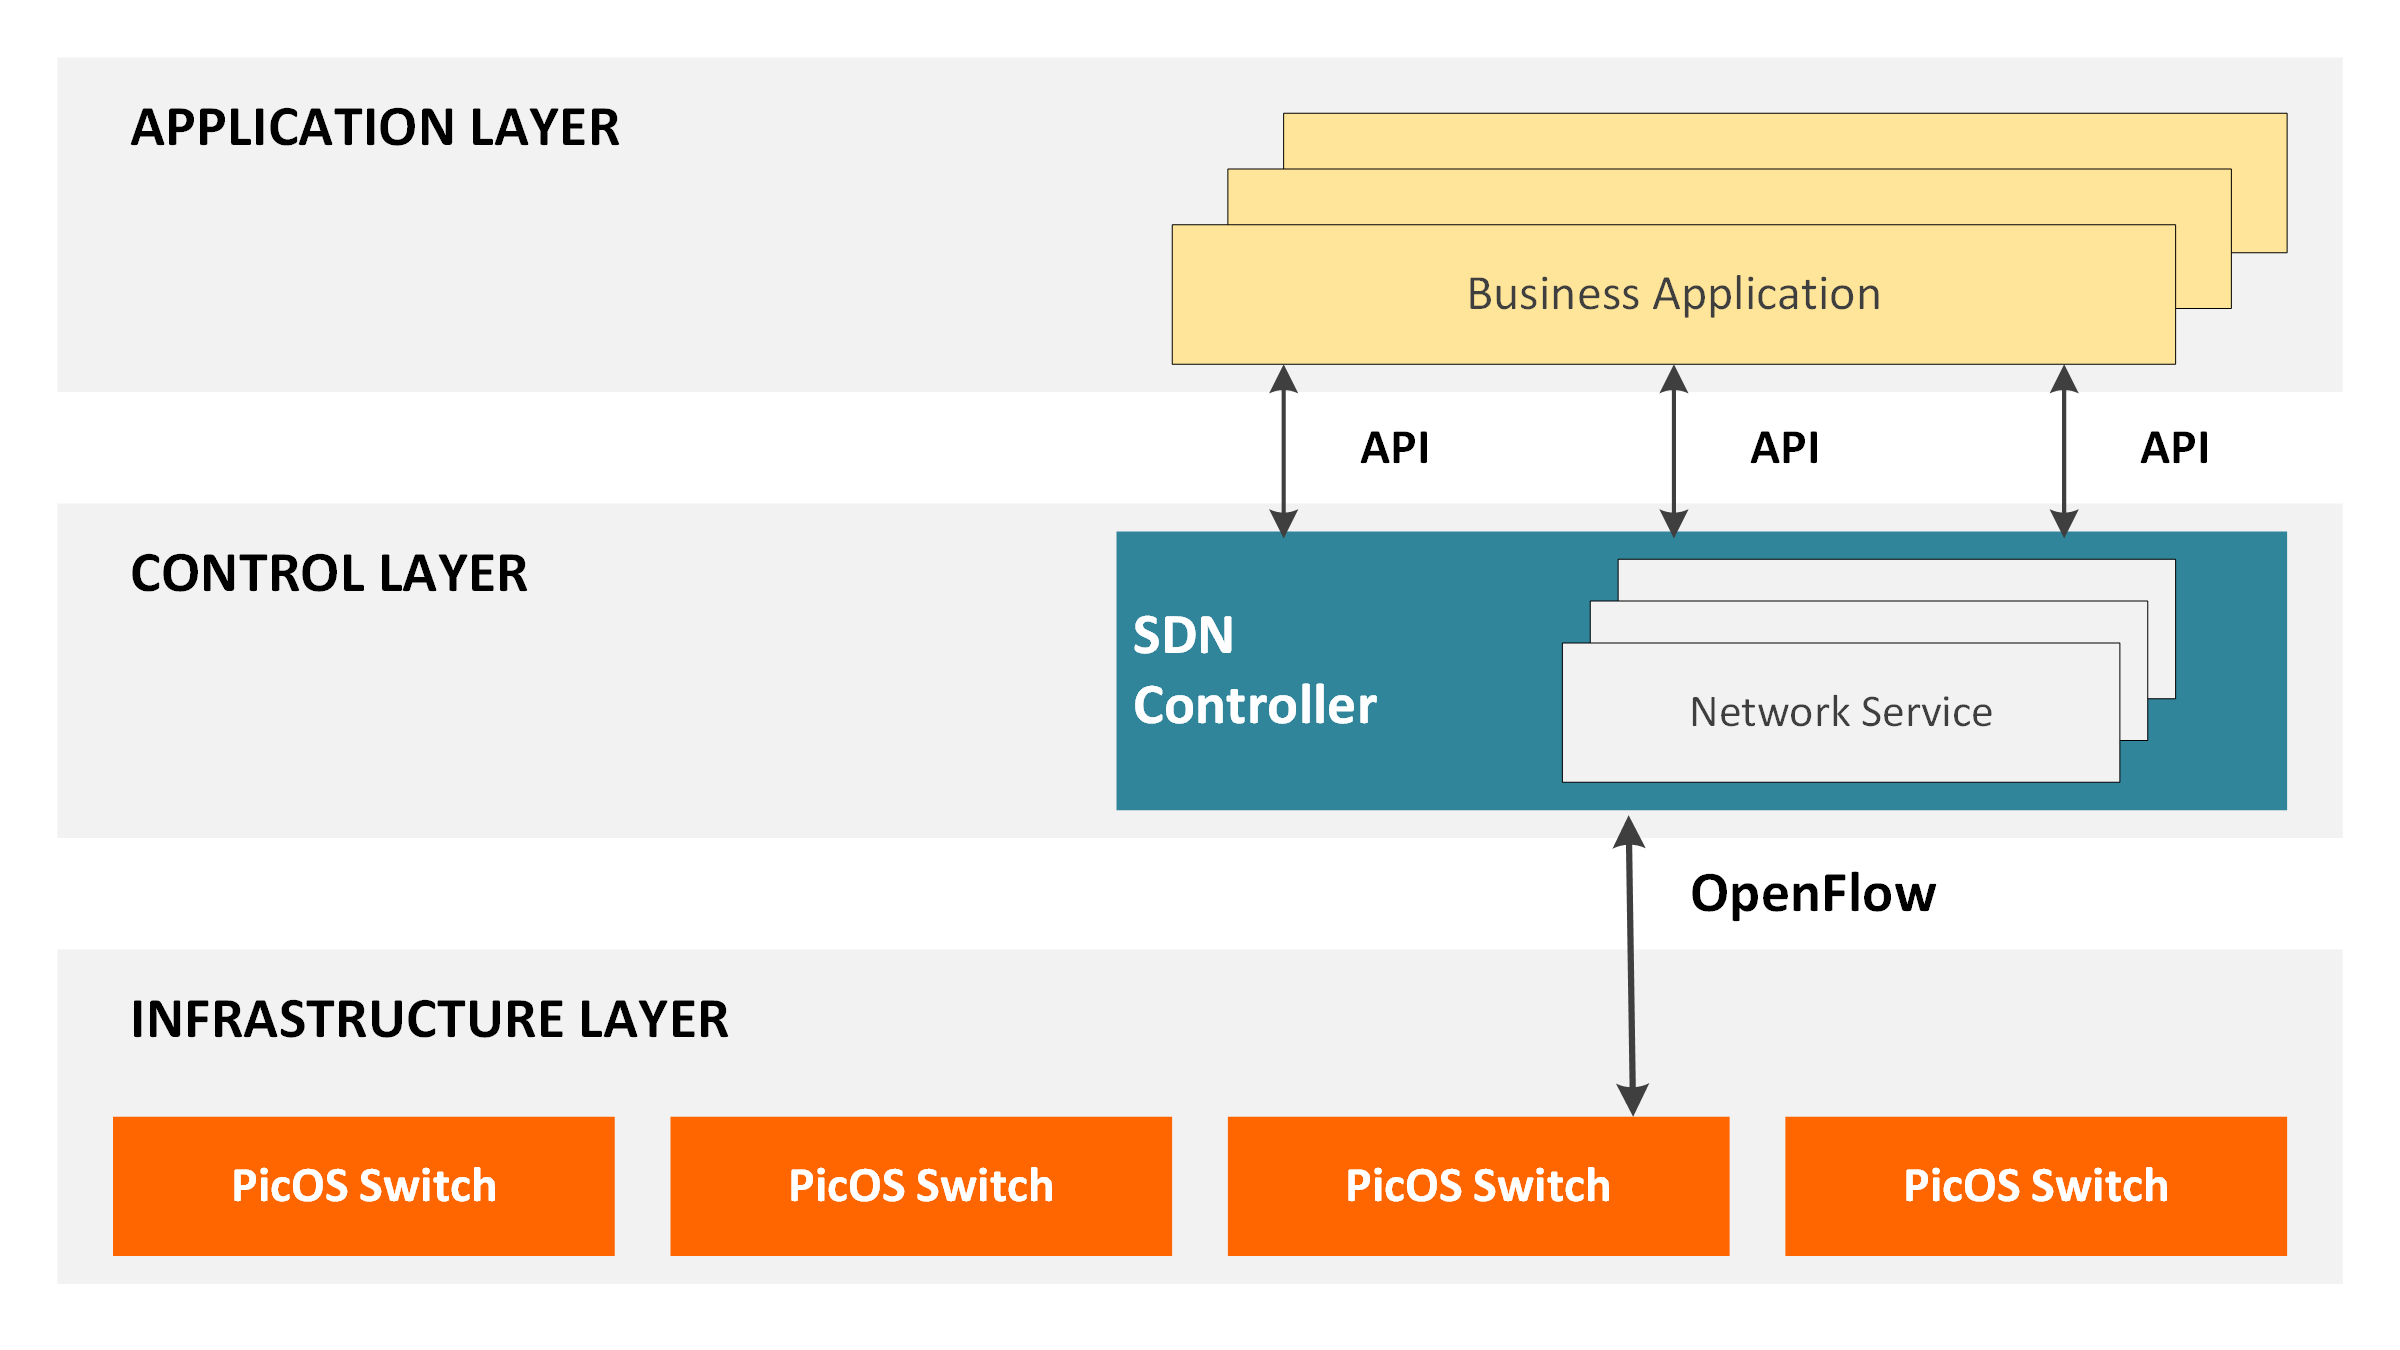
\includegraphics[width=0.8\textwidth]{arch.png}
  \caption{SDN Architecture}
  \label{fig:arch}
\end{figure}

Another mechanism we are interested in here is that the controller pulls every entry's statstics periodically to monitor the network. Using these information, a controller can estimate the throughput of each flow and the remaining bandwidth of certain links, which provides the information for scheduling of future flows and/or re-routing existing paths to guarantee QoS. \cite{traffic} is an example to illustrate this idea, and \cite{opennetmon} implemented an application to further control the monitoring process. In this work, we use emulation to simply demonstrate the concept of end-to-end throughput estimation in SDN, and show the different results when monitoring different switches in a topology.  

\begin{figure}
  \centering
  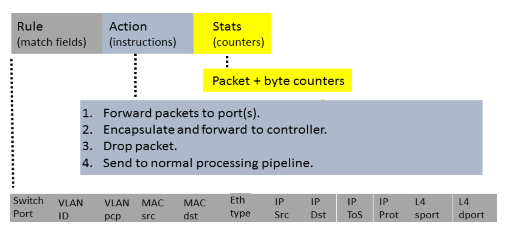
\includegraphics[width=0.8\textwidth]{openflow.png}
  \caption{OpenFlow Table Entry}
  \label{fig:openflow}
\end{figure}


\section{Estimating End-to-End Throughput}

In this work, we use the simplest way to estimate the flow throughput, which is to pull the ``number of bytes" processed by the entry and divide the elapsed time that this entry has been counting. Figure \ref{fig:onos} shows a sample web GUI of a running controller, which displays the network topology running under it. Figure \ref{fig:stats} shows the same controller's view of the table entries of the leftmost switch in the topology above. The right most two columns shows the number of packets and bytes processed by each table entry. For example, say flow A's entry has the ``BYTES" column to be X, and this entry has been installed for t seconds, then we can estimate the flow A's throughput is
\begin{equation}
\frac{X \times 8}{t} \quad bits/sec
\end{equation}

\begin{figure}
  \centering
  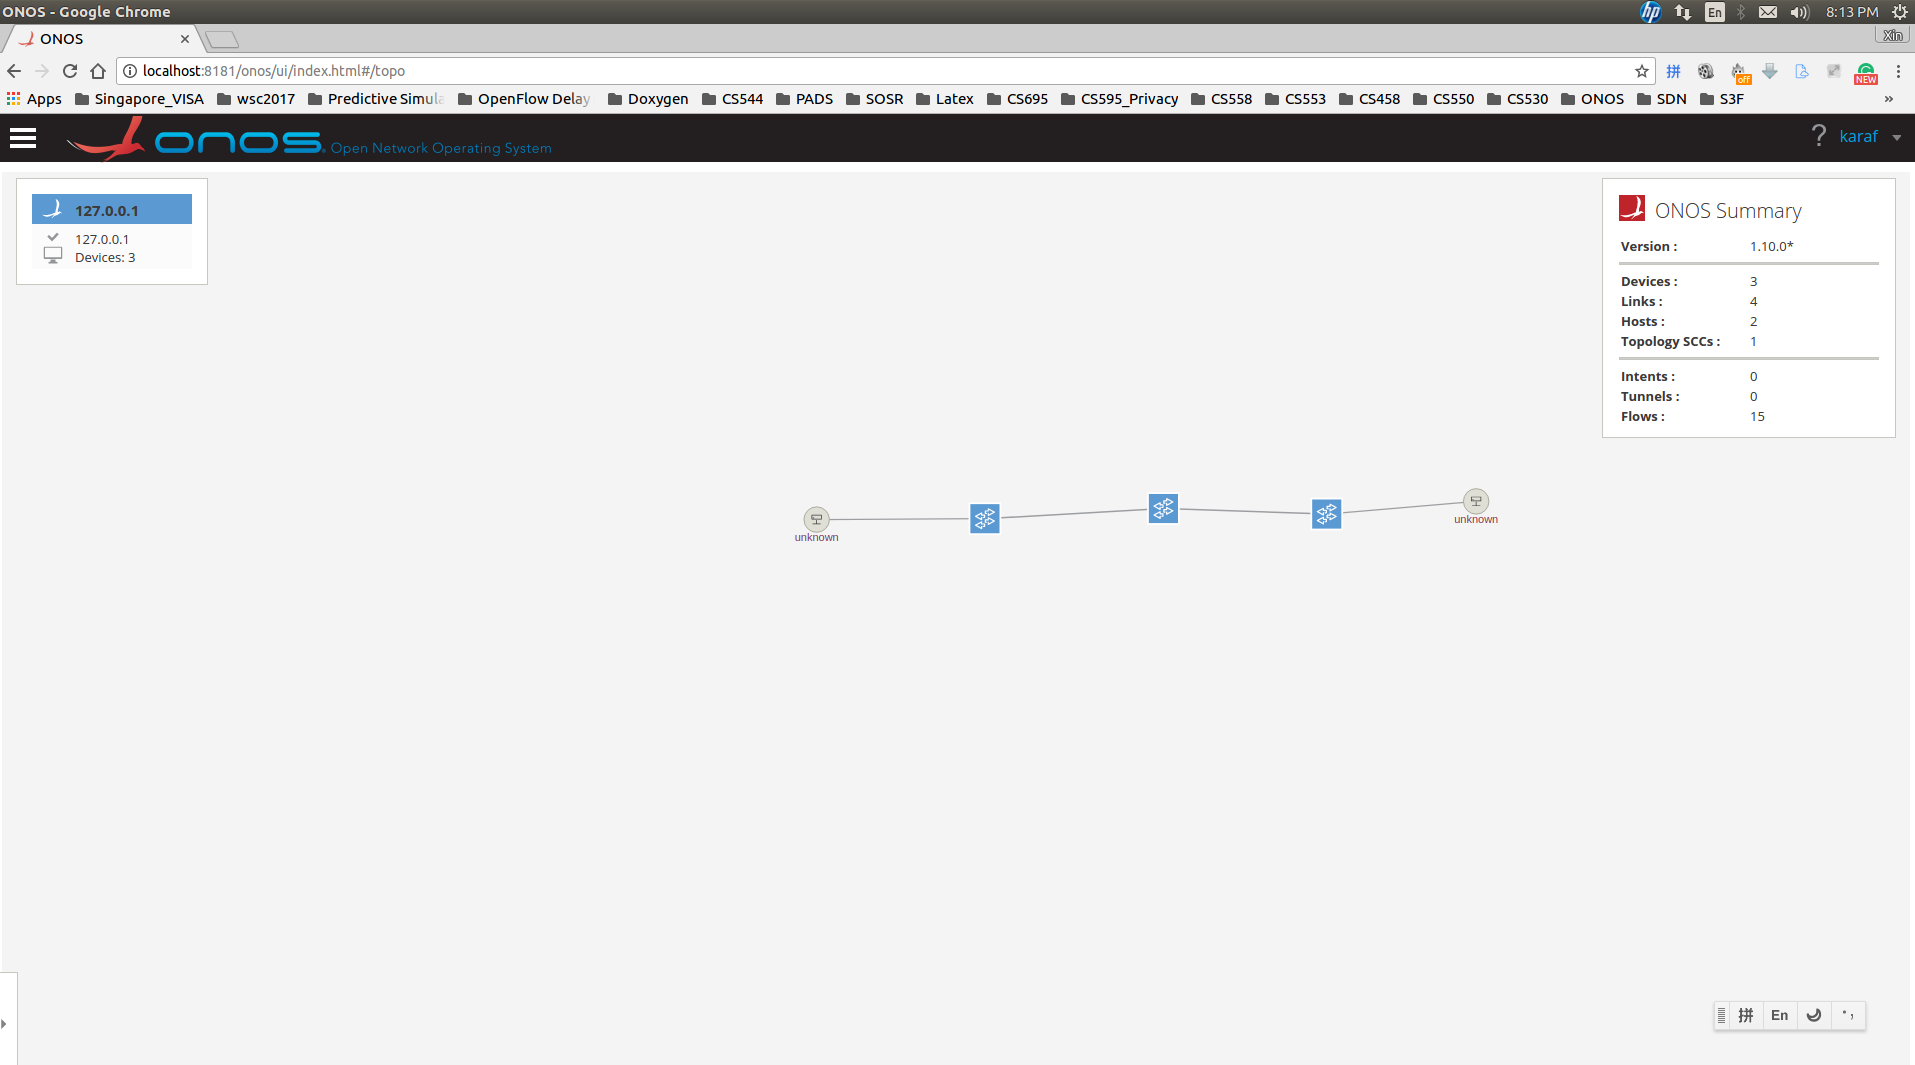
\includegraphics[width=0.9\textwidth]{onos.png}
  \caption{GUI of A Controller Showing Topology}
  \label{fig:onos}
\end{figure}

\begin{figure}
  \centering
  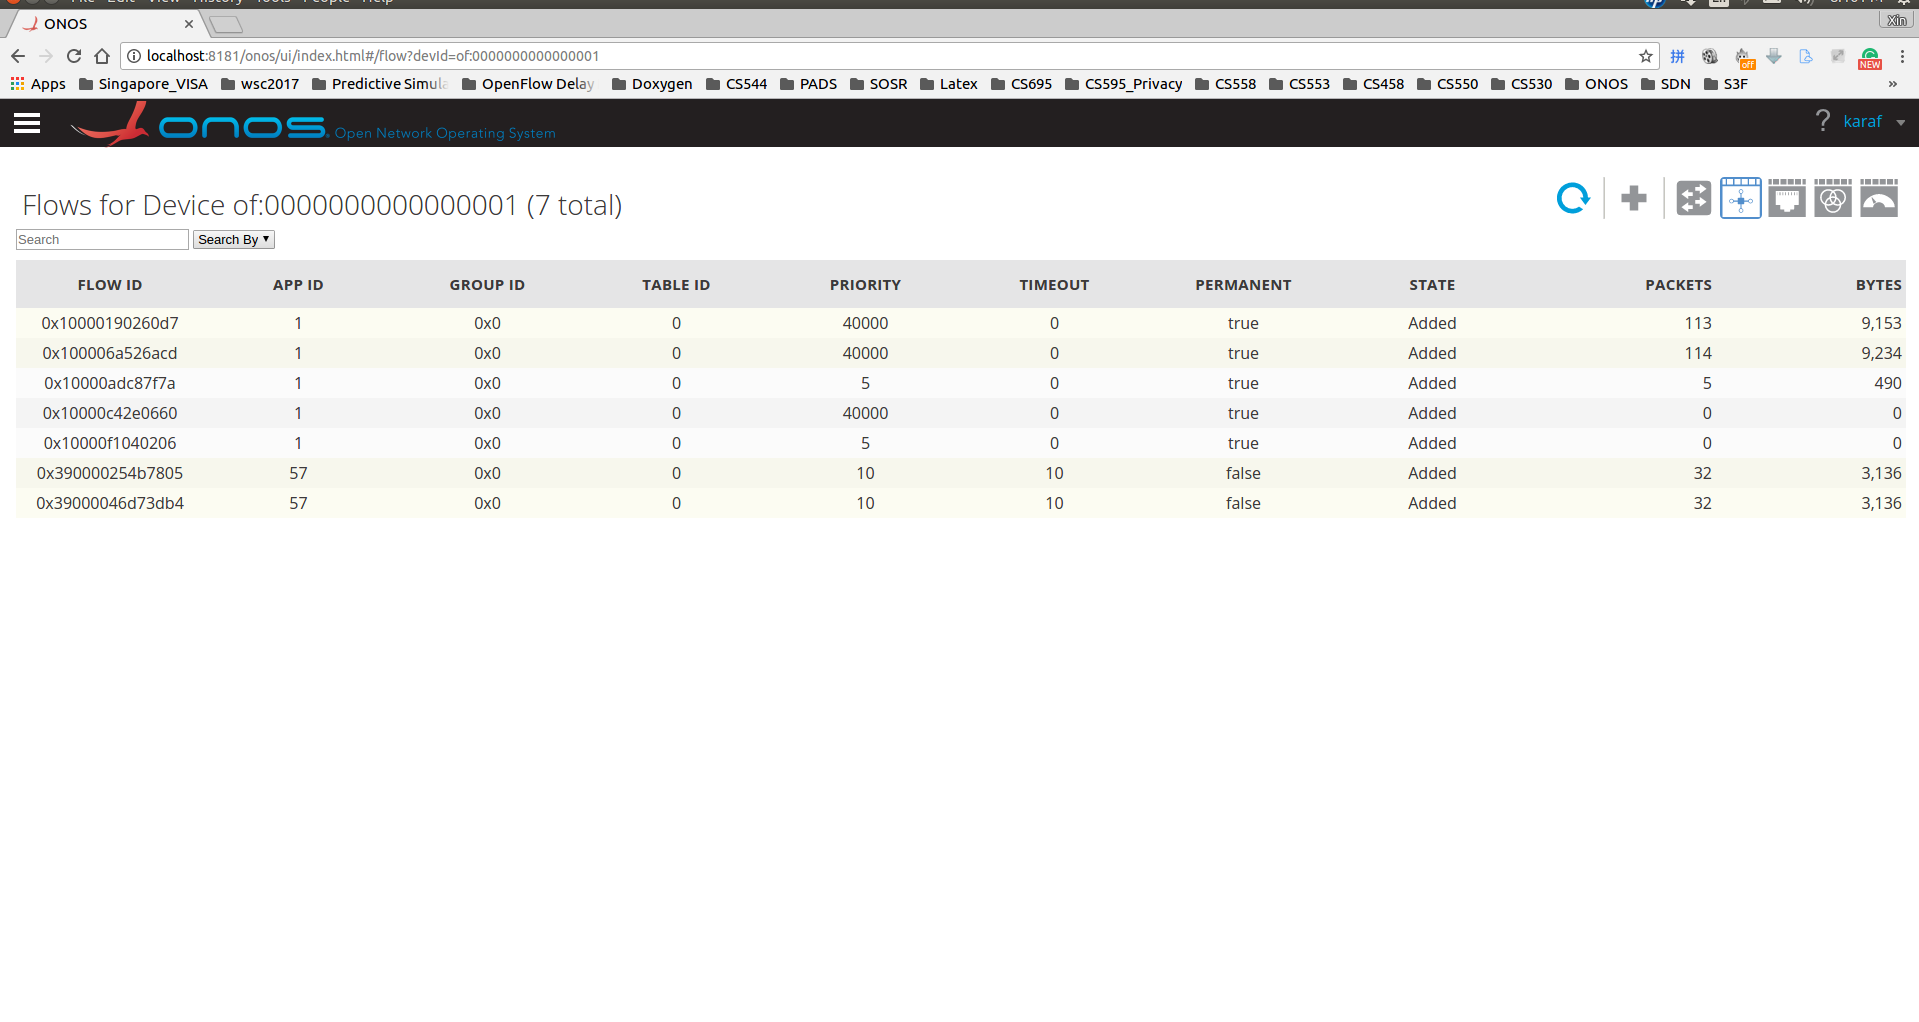
\includegraphics[width=0.9\textwidth]{stats.png}
  \caption{GUI of A Controller Showing Table Entries}
  \label{fig:stats}
\end{figure}


\section{Evaluating Estimation Accuracy Using Emulation}

To show how the esitmation works in a real network environment, we use a light-weight network emulator called Mininet \cite{mininet} to generate a simple SDN network and run iperf test on the host pairs to compare the measured throughput and estimated result.

\subsection{Mininet Emulator}

Mininet emulator use a virtualization technology called \textit{container-based virtualization}, where all the ``virtual machines" share the same Linux kernel and have their own namespaces from the application view. In Mininet, only the network namespace (i.e., network interface, eth0) is independent by each VM. As shown in Figure \ref{fig:mininet}, the target network is shown on the left hand side, where three hosts is connected by three switches. In Mininet, these three hosts are simply three Linux processes, each with a private network namespace. The switches are software switches called OpenVSwitch, and the links are configured using Linux \textit{tc} command, which contains different traffic shaping mechanism (e.g., token bucket) to guarrantee certain bandwidth and latency.

\begin{figure}
  \centering
  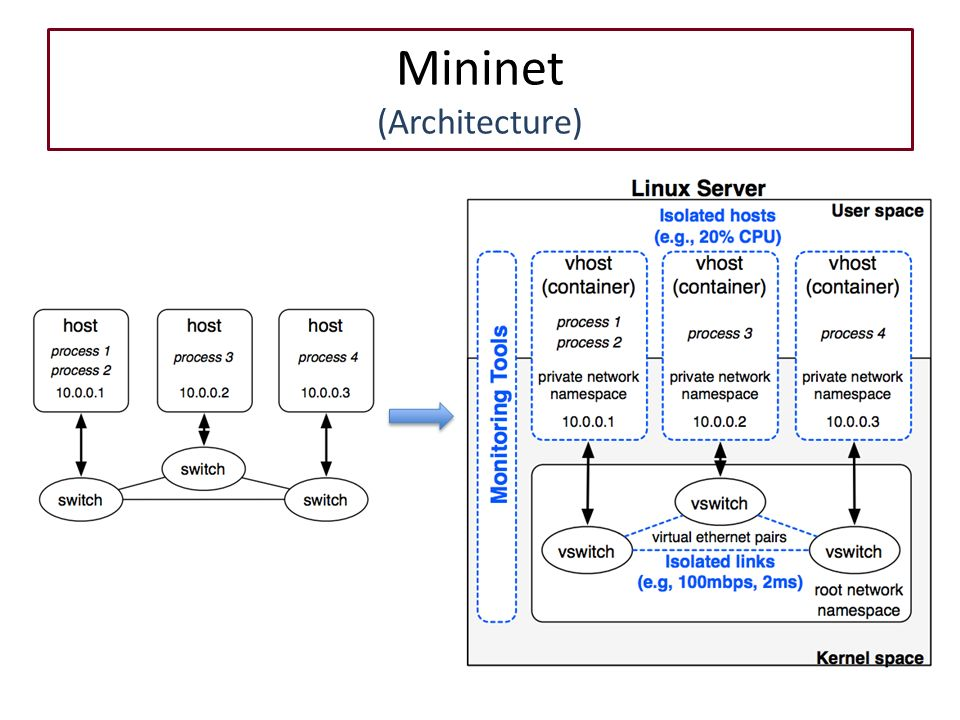
\includegraphics[width=0.7\textwidth]{mininet.jpg}
  \caption{Mininet Architecture}
  \label{fig:mininet}
\end{figure}  

Mininet provide a Python API to users, who could write scripts to generate a network and trigger the virtual hosts to execute different programs (e.g., iperf client/server program). For example, Figure \ref{fig:script} shows a code snippet of generating a simple linear topology, which will be introduced in the experiment subsection.

\begin{figure}
  \centering
  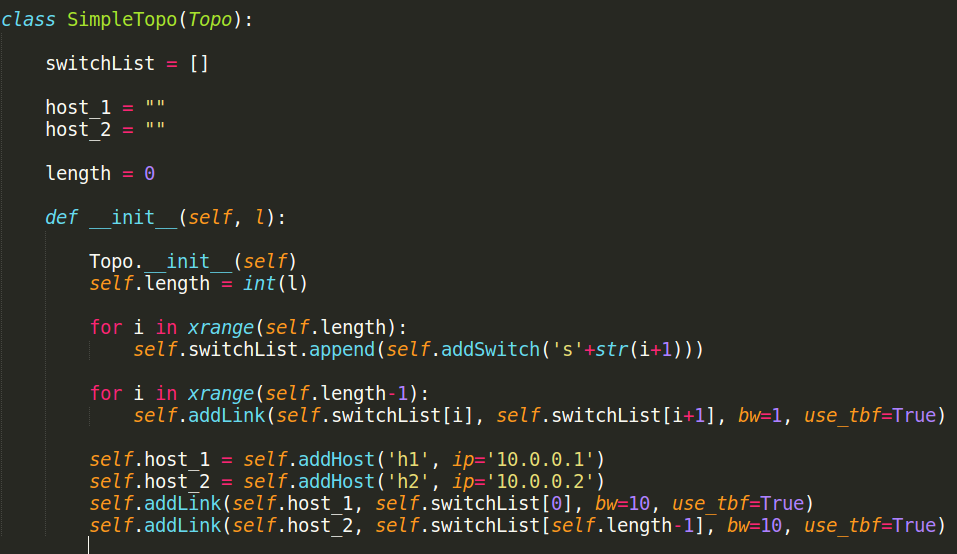
\includegraphics[width=0.8\textwidth]{script.png}
  \caption{Code Snippet}
  \label{fig:script}
\end{figure}

\subsection{Ipef Throughput Test}

Iperf \cite{iperf} is an active throughput measurement tool to evaluate the throughput between two end-hosts along a path. To begin the test, one end-host act as the server by executing ``iperf -s" command, and the other execute ``iperf -c" to generate traffic and send to the server side. There are multiple parameters can be configured, such as protocols (TCP/UDP), running time, total bytes to send, etc.

\subsection{Experiment Setup}

The experiments has three scenarios. All of them follows a linear topology, where switches form a sequence and hosts reside on the two ends. As shown in Figure \ref{fig:scenarios}, the first one is a simple linear topology of three switches, with two end-host as client/server pair. To compare with the throughput measured at the host using iperf, we monitor the flow statistics on the ingress switch and egress switch, and calculate the esitmated throughput as stated in section 3. The second scenario extend the linear topology to 100 switches, and also measure the ingress and egress switches. At last, the third scenario has the same topology as the second one, but add another pair of hosts running the iperf program at the same time, to create centention of the bandwidth. We still measure the throughput of one flow, and collect the ingress/egress switches \textbf{corresponding flow}'s stats (there are two flows at all the switches).

In all the topologies, the every link bandwidth is set 1 Mbps, and latency is set 1 msec. Each experiment is repeated 10 times.  

\begin{figure}
  \centering
  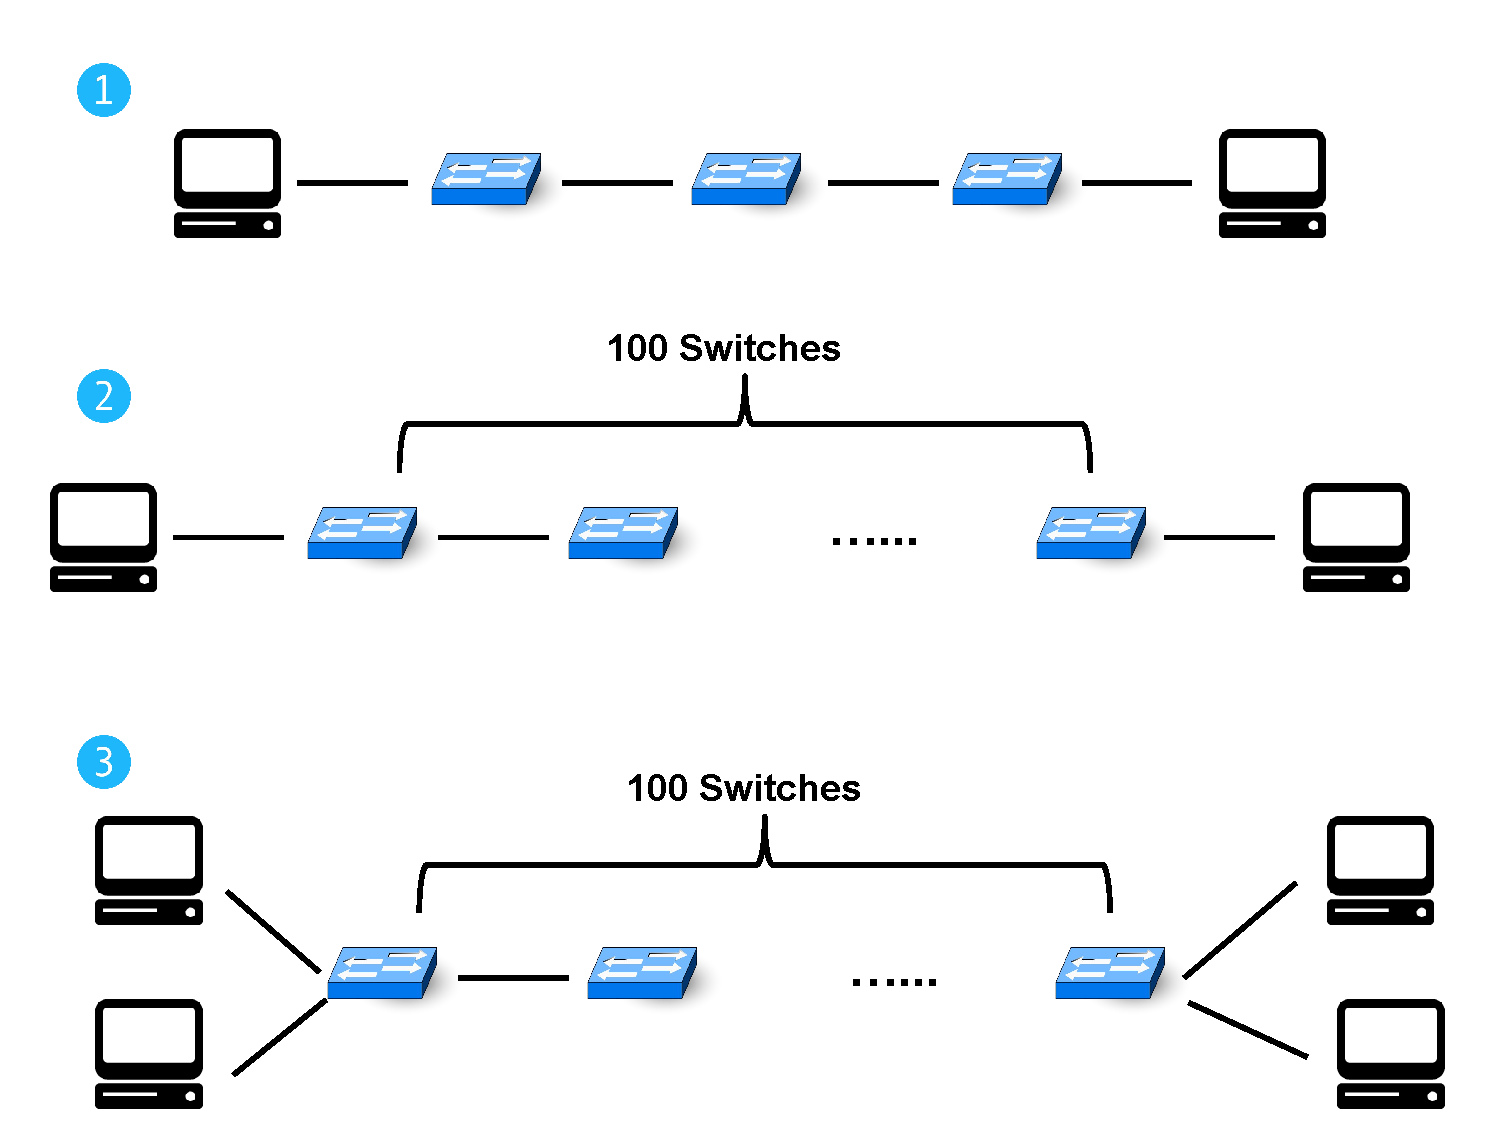
\includegraphics[width=0.7\textwidth]{Scenarios.pdf}
  \caption{Three Scenarios}
  \label{fig:scenarios}
\end{figure}

\subsection{Experiment Results and Analysis}

Following the three scenarios, we have corresponding experiment results, which are shown in Figure \ref{fig:first}, Figure \ref{fig:second}, and Figure \ref{fig:third} accordingly. Each scenario's results are illustrated in the form of (a) iperf throughput measurement at each one-second time interval, of one trial; (b) the average of measured or calculated throughput over 10 repeatitions. The ``head switch" means the throughput esitmated according to the stats on the ingress switch, while ``tail switch" measn the estimation on the egress switch. Comparing the first two scenarios, the form (a) shows that the iperf measurement nearly achieves ideal throughput (i.e., 1 Mbps), since the bandwidth of each link is set as 1 Mbps. The linear-3 has slightly better performance, which probably results from less end-to-end delay. From form (b) of the first two cases, both header and tail switch has estimation over 1 Mbps, with tail slightly closer to the iperf result. Also, the iperf nealy has no variation among the 10 trials, and tail estimation has less variation than the head version. This indicates that using the switch closer to the destination host can achieve better results. 

On the other hand, the scenario (Figure \ref{fig:third}) demonstrates fluctuated throughput on form (a), meaning the contention affects the throughput heavily. From the form (b) we can acquire the same conclusion by looking at the variation of the three throughput values. 

To further illustrate the accuracy of estimation, we use another figure, Figure \ref{fig:trial}, to show the results in the contention scenario. For each of the 10 repeatitions, we plot the iperf, header, and tail throughput values. It's clear that the estimation value is close enough to the iperf measurement, with tail results slightly better than head estimation.

\begin{figure}
\centering
\begin{subfigure}{.5\textwidth}
  \centering
  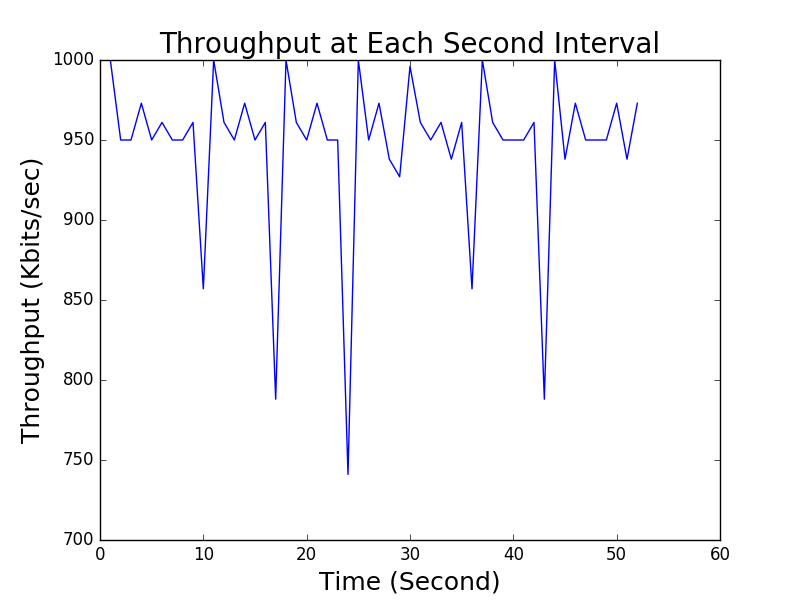
\includegraphics[width=.9\linewidth]{544_data/544_linear_5/timeline.png}
  \caption{Iperf Result Timeline}
  \label{fig:first_a}
\end{subfigure}%
\begin{subfigure}{.5\textwidth}
  \centering
  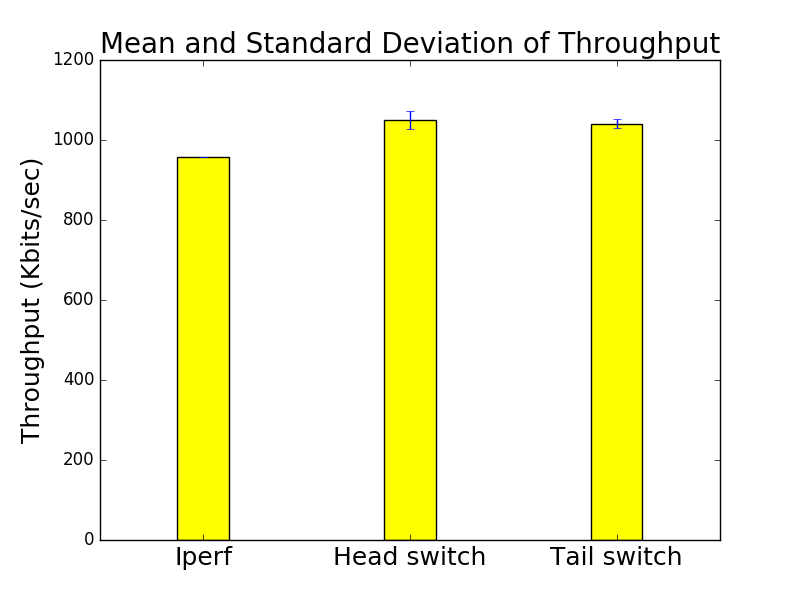
\includegraphics[width=.9\linewidth]{544_data/544_linear_5/bar.png}
  \caption{Mean Throughput}
  \label{fig:first_b}
\end{subfigure}
\caption{Result of Linear-3 Topology}
\label{fig:first}
\end{figure}

\begin{figure}
\centering
\begin{subfigure}{.5\textwidth}
  \centering
  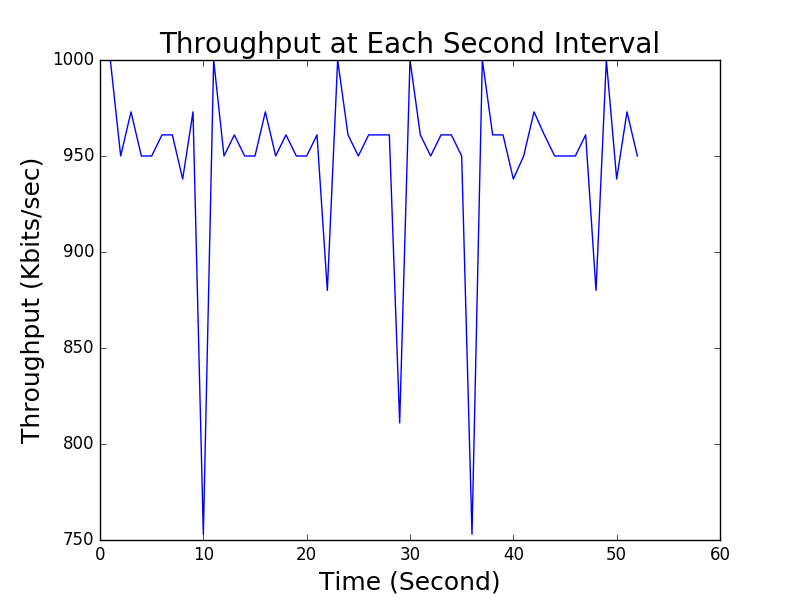
\includegraphics[width=.9\linewidth]{544_data/544_linear_100/timeline.png}
  \caption{Iperf Result Timeline}
  \label{fig:second_a}
\end{subfigure}%
\begin{subfigure}{.5\textwidth}
  \centering
  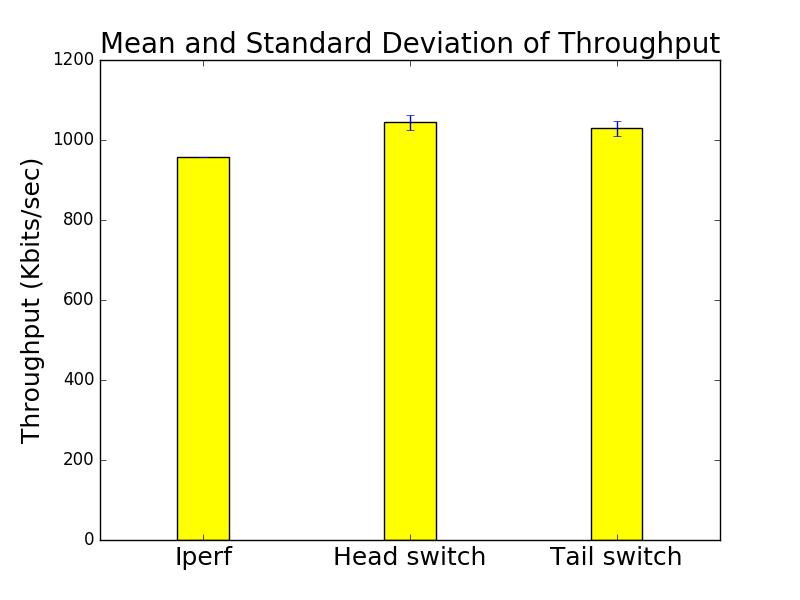
\includegraphics[width=.9\linewidth]{544_data/544_linear_100/bar.png}
  \caption{Mean Throughput}
  \label{fig:second_b}
\end{subfigure}
\caption{Result of Linear-100 Topology}
\label{fig:second}
\end{figure}

\begin{figure}
\centering
\begin{subfigure}{.5\textwidth}
  \centering
  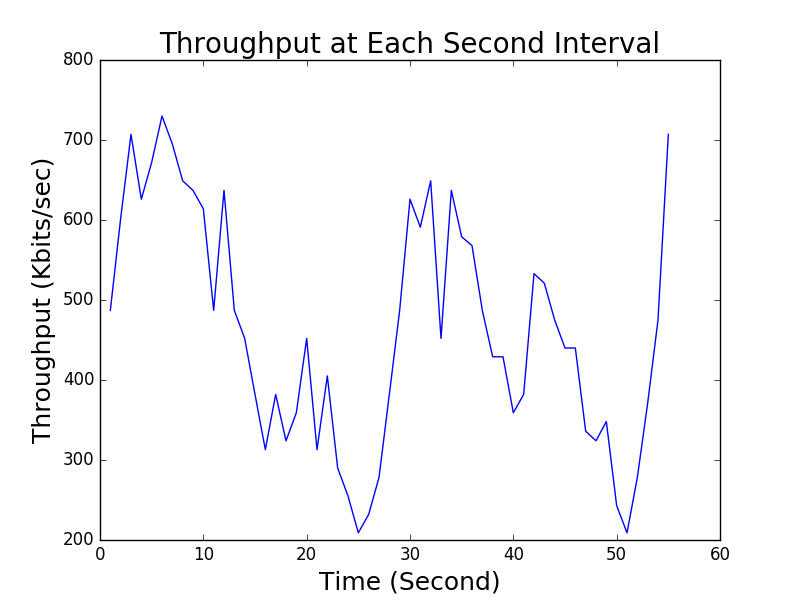
\includegraphics[width=.9\linewidth]{544_data/544_linear_100_double/timeline.png}
  \caption{Iperf Result Timeline}
  \label{fig:third_a}
\end{subfigure}%
\begin{subfigure}{.5\textwidth}
  \centering
  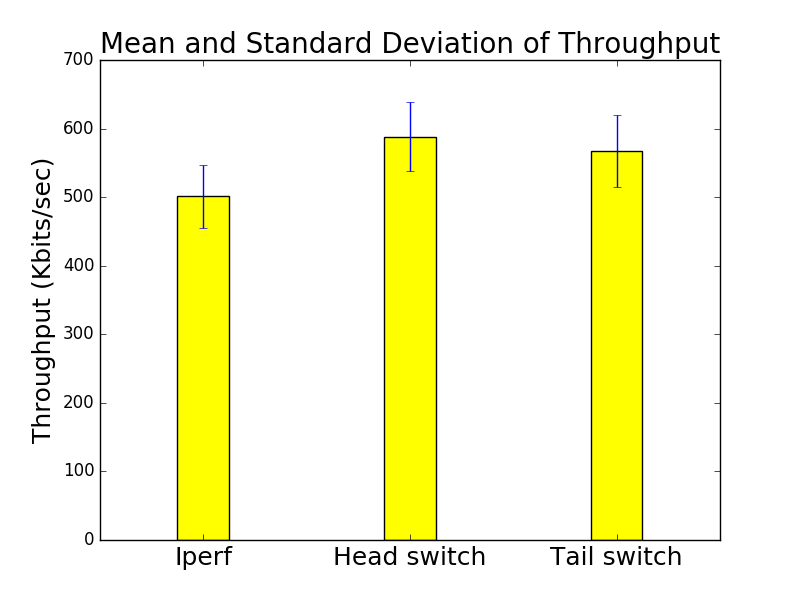
\includegraphics[width=.9\linewidth]{544_data/544_linear_100_double/bar.png}
  \caption{Mean Throughput}
  \label{fig:third_b}
\end{subfigure}
\caption{Result of Linear-100 with Contention}
\label{fig:third}
\end{figure}

\begin{figure}
  \centering
  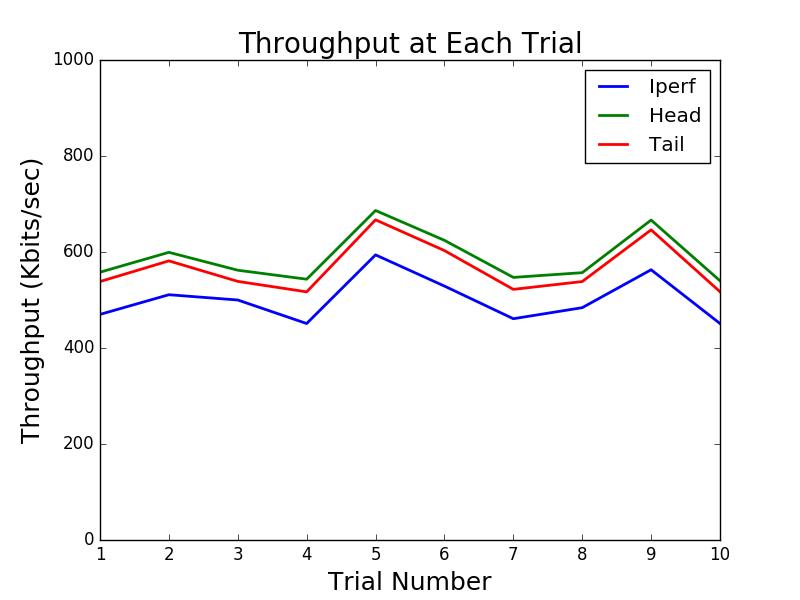
\includegraphics[width=0.7\textwidth]{544_data/trial.png}
  \caption{Linear-100 with Contention Each Trial}
  \label{fig:trial}
\end{figure}

\section{Conclusion and Future Work}

From the simple experiments in this work, we can conclude that the statistics information on the switch table entires can be used to estimate the flow's throughput, especially those close to the sink host (i.e., edge switches). However, in a large-scale and complicated network topology, choosing which switch to monitor is not a trival task. This is because the flows in the network has different source and destination hosts, and often share the same links. Also, the large number of switches makes it impossible to monitor every edge switch. Thus, given a network topology and flows, how to decide which switches to pull the stats to achieve optimal overall estimation is an interesting future work that requires further research.

\bibliography{scibib}

\bibliographystyle{Science}

\end{document}




















